\documentclass[conference]{IEEEtran}
\usepackage[utf8]{inputenc}
\usepackage[T1]{fontenc}
\usepackage{amsmath,amssymb}
\usepackage{graphicx}
\usepackage{booktabs}
\usepackage{array}
\usepackage{listings}
\usepackage{xcolor}
\usepackage{tikz}
\usetikzlibrary{positioning,arrows.meta}
\usepackage[hidelinks]{hyperref}
\graphicspath{{figures/}}

\lstdefinestyle{py}{language=Python,basicstyle=\ttfamily\scriptsize,keywordstyle=\color{blue!60!black},
  commentstyle=\color{green!40!black},stringstyle=\color{red!50!black},numbers=left,numberstyle=\tiny\color{gray},
  breaklines=true,breakatwhitespace=false,columns=fullflexible,keepspaces=true,showstringspaces=false,
  tabsize=4,frame=lines,xleftmargin=1.5em,framexleftmargin=1em}
\lstdefinestyle{log}{basicstyle=\ttfamily\tiny,breaklines=true,columns=fullflexible,frame=single,keepspaces=true}

% ---- extend the report: one \explog line per experiment (ID, status, script, output, summary)
\newcommand{\explog}[5]{#1 & #2 & \texttt{#3} & \texttt{#4} & #5 \\}

\begin{document}
\title{Uncertainty-Aware Autonomous Driving: HD-Map Localization, Behaviour Trees and Adaptive MPC}
\author{\IEEEauthorblockN{M.Tech Project Report}\IEEEauthorblockA{Python 3 / NumPy / SciPy code base; CARLA and ROS~2 integration pending}}
\maketitle

\begin{abstract}
This report documents a Python implementation of an autonomy stack: NDT + particle-filter localization on an HD map, a behaviour tree (BT) for overtaking, roundabout entry and yielding, a Frenet space-time lattice planner with QP trajectory optimisation, and pure-pursuit / Stanley / adaptive-MPC tracking. Every number reported here was produced by the scripts in this repository on \emph{synthetic} worlds; the CARLA, ROS~2, public-dataset and embedded-hardware experiments are written but \textbf{not yet run} and are listed separately. The system is a research prototype and is \textbf{not} validated for production use.
\end{abstract}
\begin{IEEEkeywords}
HD-map localization, NDT, particle filter, behaviour tree, Frenet lattice, MPC, fault injection.
\end{IEEEkeywords}

%=====================================================================
\section{Objectives}
\begin{enumerate}
\item Localize against a pre-built HD map using NDT scan matching fused in a particle filter.
\item Decide overtaking, roundabout entry and yielding with a behaviour tree that can be checked automatically.
\item Plan collision-free, smooth trajectories (lattice + QP) and track them under actuator and localization faults.
\item Quantify behaviour under injected faults and report failures honestly; keep all experiments reproducible.
\end{enumerate}

\section{System Architecture}
\begin{figure}[t]\centering
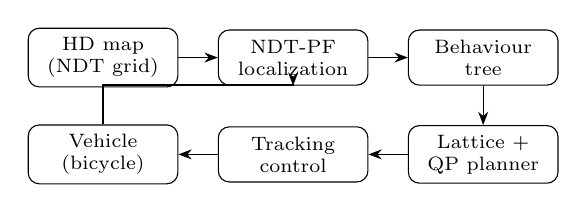
\begin{tikzpicture}[node distance=5mm,>=Stealth,box/.style={draw,rounded corners,minimum width=1.9cm,minimum height=0.7cm,align=center,font=\scriptsize}]
\node[box](map){HD map\\(NDT grid)};
\node[box,right=of map](loc){NDT-PF\\localization};
\node[box,right=of loc](bt){Behaviour\\tree};
\node[box,below=of bt](plan){Lattice +\\QP planner};
\node[box,left=of plan](ctl){Tracking\\control};
\node[box,left=of ctl](veh){Vehicle\\(bicycle)};
\draw[->](map)--(loc);\draw[->](loc)--(bt);\draw[->](bt)--(plan);\draw[->](plan)--(ctl);\draw[->](ctl)--(veh);
\draw[->](veh.north)|-++(0,0.5)-|(loc.south);
\end{tikzpicture}
\caption{Data flow. The BT outputs a target speed and lane; the planner turns them into a trajectory; the controller tracks it using the localized pose.}
\label{fig:arch}\end{figure}

\section{Methodology and Equations}
\subsection{Localization}
The HD map points are binned into cells with mean $\mu_c$ and covariance $\Sigma_c$ (regularised by $0.15I$). For pose $x=(p_x,p_y,\theta)$ and scan points $y_i$, the NDT score is
\begin{equation}S(x)=\sum_i \exp\!\big(-\tfrac12 (T(x,y_i)-\mu_{c(i)})^{\!\top}\Sigma_{c(i)}^{-1}(T(x,y_i)-\mu_{c(i)})\big).\end{equation}
Each particle is weighted $w_j\propto w_j\,(S(x_j)+\epsilon)^{\beta}$ with $\beta=0.5$. \emph{NDT-PF} adds (i) a damped-Newton NDT refinement of the weighted mean; if it scores $>0.02$ per point higher, 20\% of the lowest-weight particles are re-seeded around it, and (ii) process-noise inflation $\times3$ after 5 consecutive steps with normalised score $<0.25$.

\subsection{Behaviour tree}
Tick semantics: \emph{Selector} returns the first non-FAILURE child and resets lower-priority children; \emph{Sequence} with memory resumes the running child. Root order: roundabout $\succ$ overtake $\succ$ cruise. Overtaking starts only if the predicted pass (kinematic, duration $t_p$, ego distance $d_e$) satisfies
\begin{equation}g_{onc}-d_e-|v_{onc}|\,k\,t_p>m,\quad (k,m)=(1.3,\,40\text{ m})\end{equation}
and aborts with hysteresis $(k,m)=(1.0,15\text{ m})$ only if merging back is safe. Roundabout yielding compares the predicted arrival time $t_a$ at the conflict point with circulating-vehicle passage times $t_c$: conflict if $|t_c-t_a|<w$, $w=3$ s ($4.5$ s near the point of no return).

\subsection{Planning}
Lateral quintic and longitudinal quartic/quintic polynomials are sampled over a lattice of terminal lateral offset $l_f$, terminal speed $v_f$ and horizon $T\in\{3,4,5\}$ s, plus follow-lead terminals. Candidates are rejected on acceleration, lateral acceleration, road limits and space-time collision, then ranked by
\begin{equation}J=w_j\!\int(\dddot l^2+\dddot s^2)dt+w_T T+w_v(\dot s_f-v_{des})^2+w_l\,d(l_f,\text{lane}).\end{equation}
The best candidate is re-optimised as a bounded least-squares problem on the sample vector $x\in\{s(t),l(t)\}$:
\begin{equation}\min_x\; w_j\|D_3x\|^2+w_d\|x-x_{lat}\|^2\quad\text{s.t. } x_{lo}\le x\le x_{hi}\end{equation}
with corridor bounds from obstacle sides; the result is used only if collision-free and within dynamic limits.

\subsection{Control}
Error model about the reference with steering gain $k$: $\dot e_y=v e_\theta$, $\dot e_\theta=\tfrac{kv}{L}u$, $u=\delta-\delta_{ff}$, $\delta_{ff}=\arctan(L\kappa)/\hat k$. The MPC solves
\begin{equation}\min_u\sum_{j=1}^{N}\big(q_ye_{y,j}^2+q_\theta e_{\theta,j}^2\big)+r\|u\|^2+r_d\|\Delta u\|^2,\ |\delta|\le0.5\end{equation}
($N=15$, $\Delta t=0.1$ s). The gain is adapted by NLMS from gyro yaw rate $r_m$ with regressor $\phi=\tfrac vL\tan\delta_{filt}$:
\begin{equation}\hat k\leftarrow\hat k+\mu\,\phi\,(r_m-\hat k\phi)/(\epsilon+\phi^2).\end{equation}

\section{Implementation}
\begin{table}[t]\centering\caption{Modules (all code is listed in the appendix).}\small
\begin{tabular}{@{}p{3.3cm}p{4.6cm}@{}}\toprule File & Content\\\midrule
\texttt{localization.py} & map, NDT grid, Newton alignment, NDT-PF\\
\texttt{behavior\_tree.py} & BT library, 1-D driving world, driving tree\\
\texttt{verify\_bt.py} & structural checks, runtime monitors, grid verification\\
\texttt{planning.py} & lattice planner, QP optimiser, limit checks\\
\texttt{control.py} & reference road, bicycle model, 3 controllers\\
\texttt{closed\_loop.py} & planner$\to$controller$\to$vehicle evaluation\\
\texttt{fault\_injection.py} & localization and decision fault campaigns\\
\texttt{datasets.py} & KITTI loader, ATE/RPE (synthetic-tested only)\\
\texttt{carla\_bt\_runner.py} & CARLA adapter (not yet run)\\
\texttt{deploy/} & benchmark, ROS~2 node, Docker\\
\bottomrule\end{tabular}\end{table}

\section{Experiments Completed}
All runs: single CPU x86-64, Python 3.12.3, NumPy 2.4.4; raw logs in Appendix~\ref{app:logs}. Worlds are synthetic (Sec.~\ref{sec:limits}).

\subsection{E1: Localization (5 seeds, 412 m route)}
Sensor: 80-point scans, $\sigma=0.1$ m, 10\% outliers; gyro bias 0.01 rad/s.
\begin{table}[t]\centering\caption{E1 position RMSE [m] / converged (final error $<1$ m).}\small
\begin{tabular}{@{}lcc@{}}\toprule Method & Nominal init & Hard init (5 m, 20$^\circ$)\\\midrule
Dead reckoning & 35.01 / 0\% & 53.78 / 0\%\\
NDT only & 0.11 / 100\% & 0.49 / 100\%\\
PF (NDT likelihood) & 2.89 / 0\% & 3.04 / 0\%\\
NDT-PF & 0.30 / 100\% & 0.50 / 100\%\\\bottomrule\end{tabular}\end{table}
\begin{figure}[t]\centering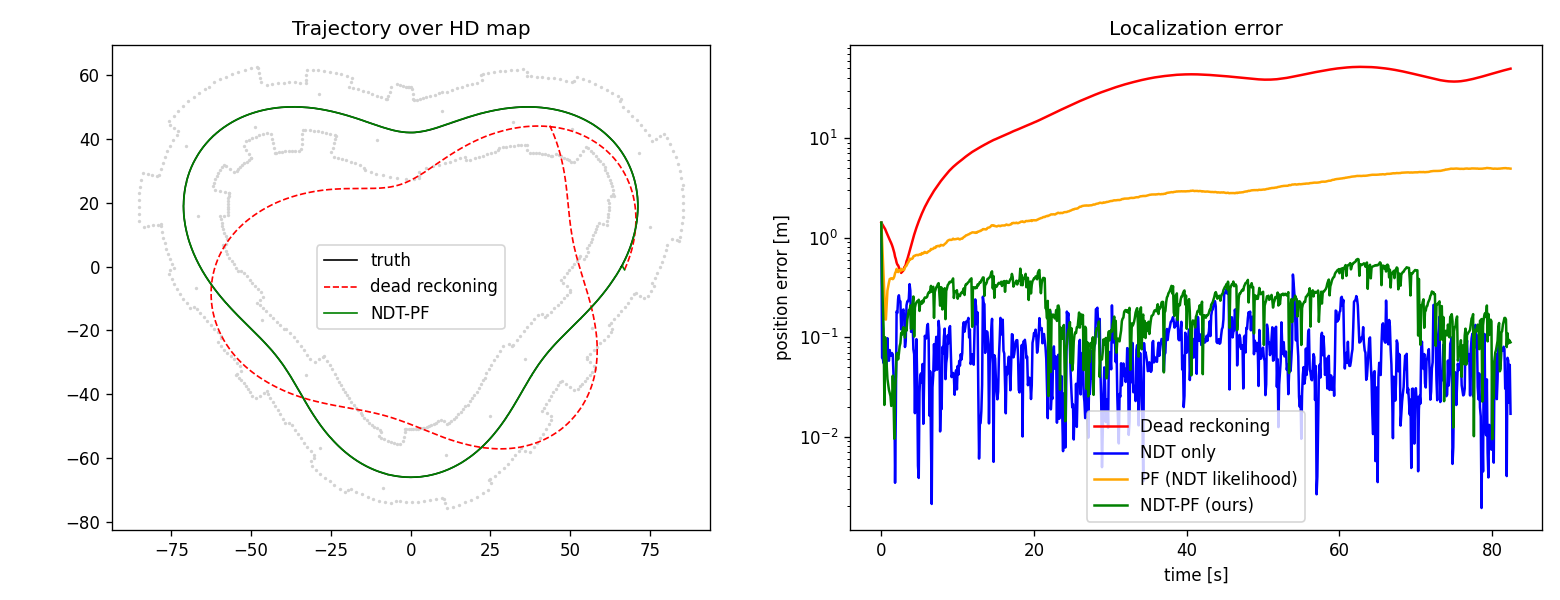
\includegraphics[width=\columnwidth]{localization_results.png}\caption{E1 trajectory and error (first seed).}\end{figure}

\subsection{E2: Behaviour tree, 300 random episodes}
Random lead speed/position, oncoming car and 2--4 circulating vehicles. Result: 100\% completion, 0\% collisions, overtakes in 72\% of episodes, mean route time 57.5 s, minimum gap median 9.2 m (5th percentile 6.4 m), waiting at the yield line in 35\% of episodes.
\begin{figure}[t]\centering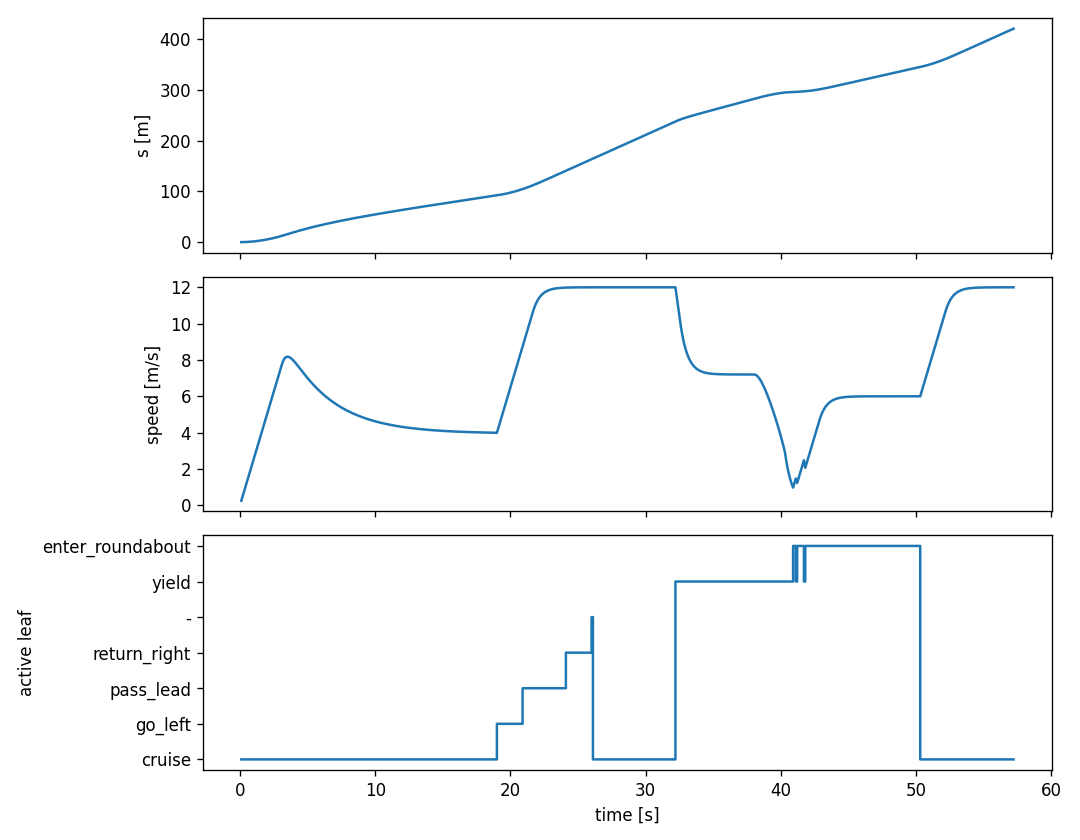
\includegraphics[width=\columnwidth]{bt_episode.png}\caption{E2 one episode: position, speed and active leaf.}\end{figure}

\subsection{E3: Behaviour-tree verification}
The tree has 11 leaves, depth 4, and a total root (last child never fails). Monitors: no collision, TTC $\ge3$ s in the oncoming lane, speed $\le8$ m/s in the roundabout, no lane change near it, one active leaf per tick. Every grid point was simulated: 3\,575 overtaking and 1\,856 roundabout scenarios gave \textbf{0 violations}. This is bounded verification over the grid and the 1-D model, not a proof for real traffic. During development the same procedure exposed defects (Table~\ref{tab:bugs}); the violation count on the overtaking grid went $148\to26\to22\to15\to135\to0$ over successive fixes.
\begin{table}[t]\centering\caption{Defects found by verification/random testing.}\label{tab:bugs}\small
\begin{tabular}{@{}p{3.6cm}p{4.2cm}@{}}\toprule Defect & Fix\\\midrule
oncoming car counted as ``passed'' when beside ego & clearance of two car lengths + 5 m\\
lead gap undefined once ego in left lane $\Rightarrow$ chatter & lane-independent gap, hysteresis\\
optimistic pass time $\Rightarrow$ unsafe abort into lead & kinematic prediction, merge-safety test\\
roundabout branch preempted a pass & pass must end before approach zone\\
no car-following in roundabout actions & speed cap applied to all actions\\
yield overshoot into conflict zone & aim 2 m short, wider window\\
scripted lead rear-ended stopped ego (model flaw) & IDM follower\\\bottomrule\end{tabular}\end{table}

\subsection{E4: Fault injection}
\begin{table}[t]\centering\caption{E4a localization faults: RMSE [m] / converged, 5 seeds. Max error 1.41 m in the first rows is the initial offset.}\small
\begin{tabular}{@{}lcc@{}}\toprule Fault & NDT only & NDT-PF\\\midrule
baseline & 0.11 / 100\% & 0.30 / 100\%\\
blackout 5 s & 0.16 / 100\% & 0.35 / 100\%\\
outliers 40\% & 0.14 / 100\% & 0.32 / 100\%\\
gyro bias 0.03 & 0.12 / 100\% & 0.21 / 100\%\\
noise 0.3 m & 0.16 / 100\% & 0.29 / 100\%\\
map change 33\% & 0.14 / 100\% & 0.41 / 100\%\\
\textbf{blackout 20 s} & 29.64 / 20\% & \textbf{2.77 / 100\%}\\
outliers 70\% & 0.23 / 100\% & 0.38 / 100\%\\
map change 67\% & 0.17 / 100\% & 0.35 / 100\%\\
severe combo & 61.09 / 0\% & 54.47 / 0\%\\\bottomrule\end{tabular}\end{table}
The score-based divergence detector (score $<0.25$ for 5 steps): recall 0.70 / false-alarm 0.11 in the 20 s blackout, recall 1.00 / false-alarm 0.19 in the severe combo, and false-alarm 0.94 at 70\% outliers (the fixed threshold is too conservative); elsewhere no step exceeded 2 m error so recall is undefined.

\begin{table}[t]\centering\caption{E4b perception faults into the BT, 200 episodes each: collision rate without / with degraded-mode supervisor.}\small
\begin{tabular}{@{}lcc@{}}\toprule Fault & No supervisor & Supervisor\\\midrule
none & 0.0\% & 0.0\%\\latency 0.5 s & 0.0\% & 0.0\%\\latency 1.0 s & 0.0\% & 0.0\%\\
oncoming dropout 3 s & \textbf{86.5\%} & 0.0\%\\oncoming speed $\times0.6$ & 0.0\% & 0.0\%\\
circulating timing $\sigma=1.5$ s & 2.0\% & 2.0\%\\\bottomrule\end{tabular}\end{table}
The supervisor flag is derived from the injected fault (idealised detector); a real detector is not implemented. Completion was 100\% in all cases.

\subsection{E5: Closed loop (planner $\to$ controller)}
Scenario: slow lead (5 m/s, $s=45$) and a parked car in the ego lane ($s=180$); target 12 m/s; 330 m. Conditions: steering gain 0.7 with 0.1 s latency, localization noise ($\sigma_{xy}=0.3$ m, $\sigma_\theta=0.01$ rad), and both.
\begin{table*}[t]\centering\caption{E5 RMS tracking error $e_y$ [m] / max $|e_y|$ [m] / minimum clearance [m]; collisions were 0 in all 16 runs. $\dagger$: did not finish within 60 s.}\small
\begin{tabular}{@{}lcccc@{}}\toprule Condition & Pure pursuit & Stanley & MPC (fixed) & Adaptive MPC\\\midrule
nominal & 0.112/0.51/1.44 & 0.070/0.26/1.29 & 0.060/0.24/1.18 & 0.060/0.24/1.17\\
gain 0.7 + latency 0.1 s & 0.160/0.61/1.39 & 0.117/0.51/1.31 & 0.090/0.36/1.24 & \textbf{0.897/3.08/0.81}\\
loc.\ noise 0.3 m & 0.193/0.64/1.04 & 0.155/0.62/0.79 & 0.145/0.62/1.35 & 0.145/0.62/1.35\\
all faults & 0.254/0.91/1.06 & 0.205/0.67/1.49 & 0.217/0.59/1.60 & \textbf{0.618/4.57/0.40}$^\dagger$\\\bottomrule\end{tabular}\end{table*}
\begin{figure}[t]\centering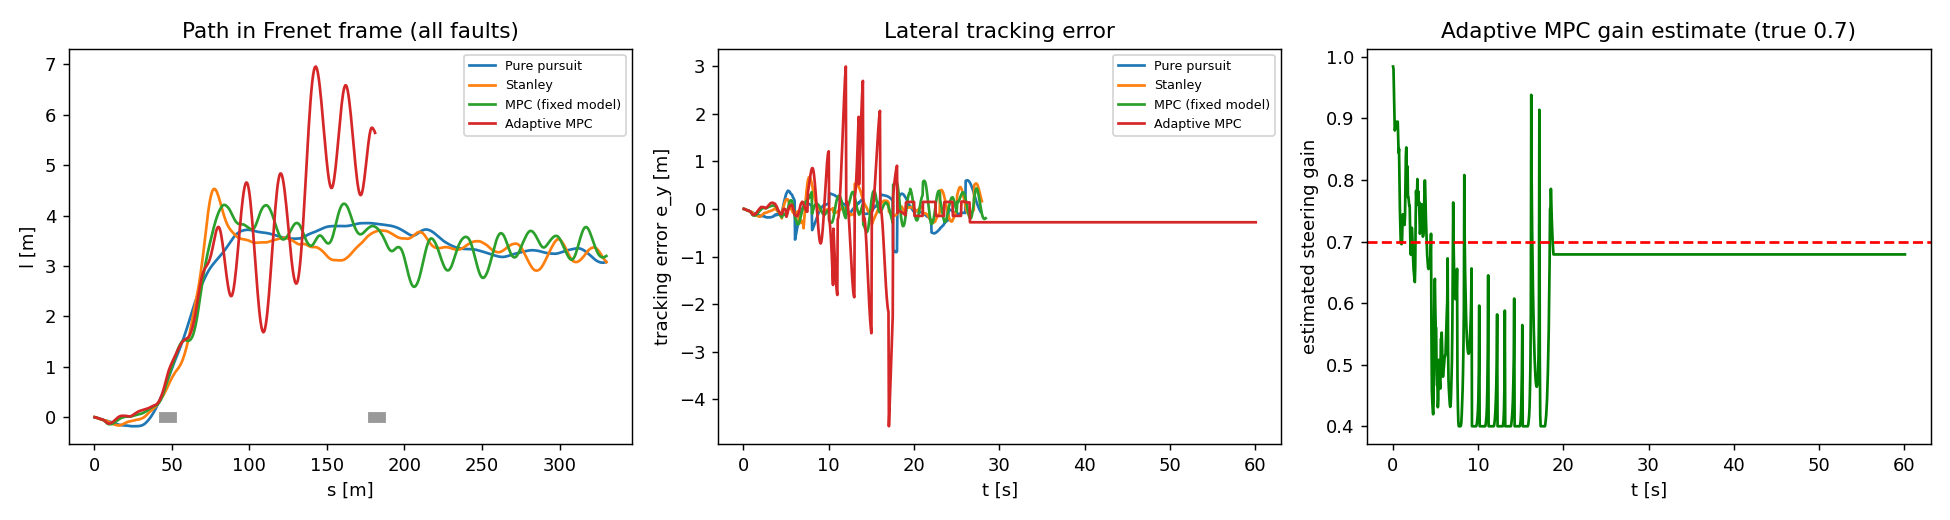
\includegraphics[width=\columnwidth]{closed_loop.png}\caption{E5 (all faults): path, tracking error, adaptive gain estimate.}\end{figure}
Observations: (i) the planner overtakes the lead and passes the parked car in all conditions; the QP result was rejected (fallback to the lattice trajectory) in 3 of 57 replans in nominal runs; (ii) fixed-model MPC gave the lowest error in three of four conditions; (iii) the gain estimator tracked the true gain without latency (0.98--1.01 nominal) but \textbf{degraded} the system with latency: the estimate fell to 0.51 (true 0.7) because the regressor ignores the 0.1 s delay, producing oscillation. This is an unresolved failure of the adaptive scheme as implemented; no benefit of adaptation was demonstrated in this study.

\subsection{E6: Latency (host CPU, not embedded)}
\begin{table}[t]\centering\caption{E6 per-call latency [ms], 60--500 calls.}\small
\begin{tabular}{@{}lcc@{}}\toprule Module & p50 & p95\\\midrule
NDT-PF cycle, 300 particles & 5.61 & 6.22\\ PF update, 1000 particles & 11.95 & 13.86\\
NDT alignment (6 iters) & 1.92 & 2.27\\ Lattice planner & 20.48 & 30.12\\
QP optimisation & 0.88 & 1.00\\ MPC step & 0.18 & 0.24\\ BT tick & 0.03 & 0.04\\\bottomrule\end{tabular}\end{table}
Latency figures predate the final planner cost retuning; re-run \texttt{deploy/embedded\_bench.py} before quoting them.

\subsection{E7: Software tests}
\texttt{tests/test\_all.py} (6 tests: BT safety, oncoming rule, NDT recovery, planner feasibility, emergency stop, controller convergence) and \texttt{tests/test\_datasets.py} pass.

\section{Experiment Log (extend here)}
\begin{table*}[t]\centering\caption{Experiment register. Add one \texttt{\textbackslash explog} line per new experiment.}\small
\scriptsize\begin{tabular}{@{}lllp{3.6cm}p{6.2cm}@{}}\toprule ID & Status & Script & Output & Summary\\\midrule
\explog{E1}{done}{run\_localization.py}{results/localization.log}{NDT-only best nominal; PF alone does not converge}
\explog{E2}{done}{behavior\_tree.py}{results/bt\_batch.log}{300 episodes, 0 collisions}
\explog{E3}{done}{verify\_bt.py}{results/bt\_verification.log}{5\,431 grid scenarios, 0 violations}
\explog{E4}{done}{fault\_injection.py}{results/fault\_injection.log}{blackout 20 s: NDT-PF recovers, NDT diverges}
\explog{E5}{done}{closed\_loop.py}{results/closed\_loop.log}{adaptive MPC fails with latency}
\explog{E6}{done}{deploy/embedded\_bench.py}{results/latency.log}{host latency only}
\explog{E7}{done}{tests/}{results/test\_all.log}{7 tests pass}
\explog{E8}{planned}{carla\_bt\_runner.py}{--}{BT in CARLA Town04, 20 seeds}
\explog{E9}{planned}{datasets.py}{--}{NDT-PF ATE on KITTI odometry seq.\ 00}
\explog{E10}{planned}{deploy/embedded\_bench.py}{--}{latency on target hardware}
\explog{E11}{planned}{control.py}{--}{model latency in gain estimator; re-run E5}
\bottomrule\end{tabular}\end{table*}

\section{Experiments Planned This Week (not yet run)}
\begin{itemize}
\item \textbf{E8 CARLA:} run \texttt{carla\_bt\_runner.py} (written, never executed) for 20 seeds; record collisions, completion, rule violations.
\item \textbf{E9 KITTI:} run NDT-PF on odometry sequence 00 with \texttt{datasets.py}; report ATE/RPE. The loader has only been tested on synthetic KITTI-format files.
\item \textbf{E10 Embedded:} run the latency benchmark on the target board and compare with the 10~Hz budget (100 ms).
\item \textbf{E11 Adaptive MPC fix:} include actuator latency in the estimator regressor, freeze adaptation when $|\phi|$ or delay is uncertain, and repeat E5.
\end{itemize}

\section{Future Experiments, Improvements and Observations}
\begin{itemize}
\item NDT-only beat NDT-PF in every non-blackout case; the particle filter's value appeared only in long sensor dropouts. Test other ambiguity cases (symmetric streets, kidnapping) before claiming more.
\item Adaptive divergence threshold for the localization monitor (false alarms 94\% at 70\% outliers); replace the idealised BT supervisor with a real perception-health monitor.
\item Circulating-traffic timing error caused 2\% collisions: use probabilistic gap acceptance.
\item Planner replans cause reference discontinuities; add warm-start continuity costs. QP rejected in 5\% of replans.
\item Replace the 1-D BT world with CARLA scenarios, add pedestrians and multi-lane roundabouts, and use real perception.
\item Report confidence intervals with more seeds (5 seeds in E1, E4a).
\end{itemize}

\section{Safety Argument (current evidence and gaps)}
\begin{table}[t]\centering\caption{Claims, evidence and status.}\small
\begin{tabular}{@{}p{2.6cm}p{3.3cm}p{1.5cm}@{}}\toprule Claim & Evidence & Status\\\midrule
BT never collides in modelled scenarios & E2, E3 (grid, 1-D) & partial\\
BT safe under perception faults & E4b & dropout needs detector\\
Localization recovers from dropouts & E4a (20 s) & partial; combo fails\\
Tracking remains safe under faults & E5 & adaptive MPC fails\\
Real-time on target & E6 host only & not shown\\
Works in real traffic & none & \textbf{open}\\\bottomrule\end{tabular}\end{table}
No hazard analysis (ISO~26262 / SOTIF), real-world data, or hardware testing exists. The prototype must not be deployed on a road vehicle.

\section{Real-World Applications}
Localization against HD maps for urban driving and shuttles; rule-based, inspectable decision making for overtaking, roundabouts and yielding; trajectory planning and tracking for ADAS/L4 research; fault-injection methods for validation of autonomy components.

\section{Limitations}\label{sec:limits}
Synthetic 2-D map with perfect data association assumptions, 1-D driving world with scripted traffic, kinematic vehicle with perfect obstacle perception (planner), 5 seeds for localization, single-CPU host timings. Results do not transfer to real roads without further work.

\begin{thebibliography}{9}
\bibitem{biber}P.~Biber, W.~Stra{\ss}er, ``The normal distributions transform: A new approach to laser scan matching,'' IROS, 2003.
\bibitem{thrun}S.~Thrun, W.~Burgard, D.~Fox, \emph{Probabilistic Robotics}, MIT Press, 2005.
\bibitem{bt}M.~Colledanchise, P.~{\"O}gren, \emph{Behavior Trees in Robotics and AI}, CRC Press, 2018.
\bibitem{werling}M.~Werling et al., ``Optimal trajectory generation for dynamic street scenarios in a Frenet frame,'' ICRA, 2010.
\bibitem{stanley}G.~Hoffmann et al., ``Autonomous automobile trajectory tracking for off-road driving,'' ACC, 2007.
\bibitem{pp}J.~Snider, ``Automatic steering methods for autonomous automobile path tracking,'' CMU-RI-TR-09-08, 2009.
\bibitem{carla}A.~Dosovitskiy et al., ``CARLA: An open urban driving simulator,'' CoRL, 2017.
\bibitem{kitti}A.~Geiger, P.~Lenz, R.~Urtasun, ``Are we ready for autonomous driving? The KITTI vision benchmark suite,'' CVPR, 2012.
\end{thebibliography}

%=====================================================================
\clearpage\onecolumn
\appendix
\section{Folder Structure and Reproduction}
\begin{lstlisting}[style=log]
sdc_project/
  main.tex  Makefile  requirements.txt  run_all.py
  localization.py  run_localization.py
  behavior_tree.py  verify_bt.py
  planning.py  control.py  closed_loop.py
  fault_injection.py  datasets.py  carla_bt_runner.py
  deploy/  embedded_bench.py  ros2_node.py  Dockerfile
  tests/   test_all.py  test_datasets.py
  figures/ localization_results.png  bt_episode.png  closed_loop.png
  results/ *.log  *.json
\end{lstlisting}
\noindent Commands: \texttt{pip install -r requirements.txt}; \texttt{python run\_all.py --quick} (tests, E1, E2, E5, E6); \texttt{python run\_all.py --full} (adds E3, E4, about 15--20 min); \texttt{make report} or compile \texttt{main.tex} in Overleaf (upload the whole folder).

\section{Source Code}
\lstinputlisting[style=py,caption={localization.py}]{localization.py}
\lstinputlisting[style=py,caption={run\_localization.py}]{run_localization.py}
\lstinputlisting[style=py,caption={behavior\_tree.py}]{behavior_tree.py}
\lstinputlisting[style=py,caption={verify\_bt.py}]{verify_bt.py}
\lstinputlisting[style=py,caption={planning.py}]{planning.py}
\lstinputlisting[style=py,caption={control.py}]{control.py}
\lstinputlisting[style=py,caption={closed\_loop.py}]{closed_loop.py}
\lstinputlisting[style=py,caption={fault\_injection.py}]{fault_injection.py}
\lstinputlisting[style=py,caption={datasets.py}]{datasets.py}
\lstinputlisting[style=py,caption={deploy/embedded\_bench.py}]{deploy/embedded_bench.py}
\lstinputlisting[style=py,caption={carla\_bt\_runner.py (not yet executed)}]{carla_bt_runner.py}
\lstinputlisting[style=py,caption={deploy/ros2\_node.py (not yet executed)}]{deploy/ros2_node.py}
\lstinputlisting[style=py,caption={tests/test\_all.py}]{tests/test_all.py}
\lstinputlisting[style=py,caption={tests/test\_datasets.py}]{tests/test_datasets.py}
\lstinputlisting[style=py,caption={run\_all.py}]{run_all.py}
\lstinputlisting[style=log,caption={deploy/Dockerfile}]{deploy/Dockerfile}

\section{Raw Experiment Logs}\label{app:logs}
\lstinputlisting[style=log,caption={results/localization.log}]{results/localization.log}
\lstinputlisting[style=log,caption={results/bt\_batch.log}]{results/bt_batch.log}
\lstinputlisting[style=log,caption={results/bt\_verification.log}]{results/bt_verification.log}
\lstinputlisting[style=log,caption={results/fault\_injection.log}]{results/fault_injection.log}
\lstinputlisting[style=log,caption={results/closed\_loop.log}]{results/closed_loop.log}
\lstinputlisting[style=log,caption={results/latency.log}]{results/latency.log}
\lstinputlisting[style=log,caption={results/test\_all.log}]{results/test_all.log}
\end{document}
